\documentclass[10pt]{beamer}

\usetheme[progressbar=frametitle]{metropolis}
\usepackage{appendixnumberbeamer}

\usepackage{booktabs}
\usepackage[scale=2]{ccicons}

\usepackage{pgfplots}
\usepgfplotslibrary{dateplot}

\usepackage{xspace}
\newcommand{\themename}{\textbf{\textsc{metropolis}}\xspace}

\title{The Pinksy-Rinzel Model and Parameter Estimation}

\date{\today}

\author{Matthias Heinkenschloss, Arjun Sethi-Olowin}
\institute{Department of Computational and Applied Mathematics and Operations Research\\Rice University, Houston, Texas}
% \titlegraphic{\hfill\includegraphics[height=1.5cm]{logo.pdf}}

\begin{document}

\maketitle

\begin{frame}{Table of contents}
  \setbeamertemplate{section in toc}[sections numbered]
  \tableofcontents%[hideallsubsections]
\end{frame}

\section[Pinsky-Rinzel Model]{Pinsky-Rinzel Model}

\begin{frame}[fragile]{Overview of the Model}

    \begin{itemize}
        \item A system of differential equations
        \item Models behavior of the CA3 neurons in the hippocampus
        \item Split into a somatic compartment and a dendritic compartment
    \end{itemize}
    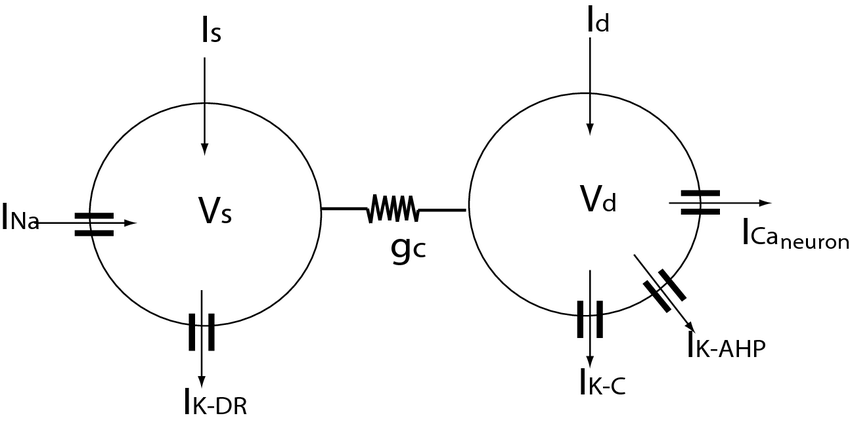
\includegraphics[width=0.7\textwidth]{Latex/Figures/prmodel_figs/Schematic_Pinsky-Rinzel_Model.png}
\end{frame}

\begin{frame}{Two-Compartment Model}
    We first define a series of equations that represent the ionic currents.
    \alt<2>
    {
    \begin{align*}
         \textcolor{red}{I_{Leak}}(\textcolor{red}{V_s}(t)) &= \textcolor{blue}{g_L}(\textcolor{red}{V_s}(t)-\textcolor{blue}{V_L})\\
         \textcolor{red}{I_{Leak}}(\textcolor{red}{V_d}(t)) &= \textcolor{blue}{g_L}(\textcolor{red}{V_d}(t)-\textcolor{blue}{V_L})\\
         \textcolor{red}{I_{Na}}(\textcolor{red}{V_s}(t)) &= \textcolor{blue}{g_{Na}}(\textcolor{red}{m_\infty}(\textcolor{red}{V_s}(t)))^2\textcolor{red}{h}(t)(\textcolor{red}{V_s}(t)-\textcolor{blue}{V_{Na}})\\
         \textcolor{red}{I_{K-DR}}(\textcolor{red}{V_s}(t)) &= \textcolor{blue}{g_{K-DR}}\textcolor{red}{n}(t)(\textcolor{red}{V_s}(t)-\textcolor{blue}{V_k})\\
         \textcolor{red}{I_{Ca}}(\textcolor{red}{V_d}(t)) &= \textcolor{blue}{g_{Ca}}(\textcolor{red}{s}(t))^2(\textcolor{red}{V_d}(t)-\textcolor{blue}{V_{Ca}})\\
         \textcolor{red}{I_{K-C}}(\textcolor{red}{V_d}(t)) &= \textcolor{blue}{g_{K-C}}\textcolor{red}{c}(t)\textcolor{red}{\chi}(\textcolor{red}{Ca}(t))(\textcolor{red}{V_d}(t)-\textcolor{blue}{V_k})\\
         \textcolor{red}{I_{K-AHP}}(\textcolor{red}{V_d}(t)) &= \textcolor{blue}{g_{K-AHP}}\textcolor{red}{q(t)}(\textcolor{red}{V_d}(t)-\textcolor{blue}{V_k})
     \end{align*}
     
    We define the addition functions as
    \begin{align*}
        \frac{d}{dt}\textcolor{red}{Ca}(t) &= -0.13\textcolor{red}{I_{Ca}}-0.0075\textcolor{red}{Ca(t)}\\
        \frac{d}{dt}\textcolor{red}{y}(t) &= \frac{(\textcolor{red}{y_\infty}(\textcolor{red}{U})-\textcolor{red}{y}(t))}{\textcolor{red}{\tau_y}(\textcolor{red}{U})}
    \end{align*}
    where $U=V_s(t)$ for $y=h,n$; $U=V_d(t)$ for $y=s,c$; $U=Ca(t)$ for $y=q$. $y_\infty$ and $\tau_y$ are given in the appendix.
    }
    {
    \begin{align*}
         I_{Leak}(V_s(t)) &= g_L(V_s(t)-V_L)\\
         I_{Leak}(V_d(t)) &= g_L(V_d(t)-V_L)\\
         I_{Na}(V_d(t)) &= g_{Na}m_\infty^2(V_s(t))h(V_s(t)-V_{Na})\\
         I_{K-DR}(V_s(t)) &= g_{K-DR}n(V_s(t)-V_k)\\
         I_{Ca}(V_d(t)) &= g_{Ca}s^2(V_d(t)-V_{Ca})\\
         I_{K-C}(V_d(t)) &= g_{K-C}c\chi(Ca)(V_d(t)-V_k)\\
         I_{K-AHP}(V_d(t)) &= g_{K-AHP}q(V_d(t)-V_k)
    \end{align*}
    
    We define the addition functions as
    \begin{align*}
        \frac{d}{dt}Ca(t) &= -0.13I_{Ca}-0.0075Ca(t)\\
        \frac{d}{dt}y(t) &= \frac{(y_\infty(U)-y(t))}{\tau_y(U)}
    \end{align*}
    where $U=V_s(t)$ for $y=h,n$; $U=V_d(t)$ for $y=s,c$; $U=Ca(t)$ for $y=q$. $y_\infty$ and $\tau_y$ are given in the appendix.
    }
\end{frame}


\begin{frame}{Two-Compartment Model Cont.}
    Now we can define the current balance equations between the somatic and dendritic compartments. 
    \begin{align*}
    C_m\frac{d}{dt}V_s &= -I_{Leak}(V_s) - I_{Na} - I_{K-DR} + \frac{g_c(V_d-V_s) + I_s}{p}\\
    C_m\frac{d}{dt}V_d &= -I_{Leak}(V_d) - I_{Ca}- I_{K-AHP} - I_{K-C} - \frac{I_{Syn}+g_c(V_s-V_d)+I_d}{1-p}
    \end{align*}
    where $I_{Syn}$ is a function which models a multi cellular system and is fully provided in the appendix. 
\end{frame}
    
   
\begin{frame}{Constant values and initial conditions}
    We give initial values for the functions above and values for the constants. 
    \begin{columns}
    \column{0.3\textwidth}
        \textbf{Parameters}
        \begin{align*}
            g_{Na} &\\
            g_{K-DR} &\\
            g_{L} &\\
            g_{Ca} &\\
            g_{K-AHP} &\\
            g_{K-C} &\\
            g_c &
        \end{align*}
    \column{0.3\textwidth}
        \textbf{Constants}
        \begin{align*}
            C_m &= 3\\
            p &= 0.5\\
            I_s &= 0.25\\
            V_{Na} &= 120\\
            V_{k} &= -15\\
            V_{L} &= 0\\
            V_{Ca} &= 140\\
            V_{syn} &= 60
        \end{align*}
    \column{0.3\textwidth}
        \textbf{Initial values}
        \begin{align*}
            V_s(0) &= -4.6\\
            V_d(0) &= -4.5\\
            h(0) &= 0.001\\
            n(0) &= 0.999\\
            s(0) &= 0.009\\
            c(0) &= 0.007\\
            q(0) &= 0.010\\
            Ca(0) &= 0.2
        \end{align*}
    \end{columns}
\end{frame}



\section{Two Compartment Numerical Simulations}

\begin{frame}{Code}
	We know constants which are...\\
    have some parameters which are constant in time, but value is undetermined\\
    functions?
\end{frame}

\begin{frame}{Visualizations for Functions}
    graphics of the functions
\end{frame}

\section{Two-Compartment Pyomo Parameter Estimation}

\begin{frame}{Simulation}
    Simulation code where we provide parameter values to understand how various functions in the model change
\end{frame}

\begin{frame}{Pyomo}
    Pyomo code solves parameters to minimize error for function values over time compared to collected data
\end{frame}

\section{Conclusion}

\begin{frame}{Summary}
    
\end{frame}

\begin{frame}{Next Steps}
    Pyomo stuff
\end{frame}
    



\appendix

\begin{frame}{References}

    references here
    
\end{frame}

\end{document}
